%%%%%%%%%%%%%%%%%%%%%%%%%%%%%%%%%%%%%%%%%
% a0poster Portrait Poster
% LaTeX Template
% Version 1.0 (22/06/13)
%
% The a0poster class was created by:
% Gerlinde Kettl and Matthias Weiser (tex@kettl.de)
% 
% This template has been downloaded from:
% http://www.LaTeXTemplates.com
%
% License:
% CC BY-NC-SA 3.0 (http://creativecommons.org/licenses/by-nc-sa/3.0/)
%
%%%%%%%%%%%%%%%%%%%%%%%%%%%%%%%%%%%%%%%%%

%----------------------------------------------------------------------------------------
%	PACKAGES AND OTHER DOCUMENT CONFIGURATIONS
%----------------------------------------------------------------------------------------

\documentclass[a0,portrait]{a0poster}
\usepackage{multicol}
\usepackage[svgnames]{xcolor}
\usepackage{times}
\usepackage{graphicx}
\graphicspath{{figures/}}
\usepackage{booktabs}
\usepackage[font=small,labelfont=bf]{caption}
\usepackage{amsfonts, amsmath, amsthm, amssymb}
\usepackage{wrapfig}
\usepackage{indentfirst}
\usepackage{enumitem}
\usepackage{tikz}
\usetikzlibrary{shapes.geometric, arrows, positioning, fit, backgrounds}
\usepackage[style=authoryear,backend=biber,heading=bibintoc]{biblatex}
\addbibresource{references.bib}

% Define ARDC colors
\definecolor{ARDCBlue}{RGB}{0,159,218}
\definecolor{ARDCPink}{RGB}{236,0,140}
\definecolor{ARDCYellow}{RGB}{255,194,14}
\definecolor{ARDCPurple}{RGB}{146,39,143}
\definecolor{DarkGrey}{RGB}{64,64,64}

% Set margins
\setlength{\topmargin}{1cm}
\setlength{\oddsidemargin}{1cm}
\setlength{\evensidemargin}{1cm}
\setlength{\textwidth}{0.95\paperwidth}
\setlength{\textheight}{0.95\paperheight}
\setlist[enumerate]{leftmargin=2em}

% Increase first-line indent
\setlength{\parindent}{2em}

\begin{document}

%----------------------------------------------------------------------------------------
% POSTER HEADER
%----------------------------------------------------------------------------------------
\noindent\begin{minipage}[t]{\linewidth}
\Huge \color{ARDCBlue} \textbf{Improving Practices for Persistently Recording the CARE Principles} \color{Black}\\[0.3cm]
\LARGE\textit{for Collections of Place-based Research Samples, Observations and Instrument Measurements}\\[1cm]
\end{minipage}



\noindent\begin{minipage}[t]{0.75\linewidth}
\Large \textbf{Lesley A Wyborn\textsuperscript{1}, Erin Robinson\textsuperscript{2}, Rebecca Farrington\textsuperscript{3}, Shawn Ross\textsuperscript{4}, Natasha Simons\textsuperscript{4}}\\[0.5cm]
\large \textsuperscript{1}Australian National University, Canberra, ACT, Australia\\
\textsuperscript{2}Self Employed, Boulder, United States\\
\textsuperscript{3}AuScope Ltd, Melbourne, VIC, Australia\\
\textsuperscript{4}Australian Research Data Commons, Australia
\end{minipage}%
\begin{minipage}[t]{0.25\linewidth}
\raggedleft
\raisebox{\dimexpr-\height+\ht\strutbox\relax}{
\includegraphics[width=0.95\linewidth]{ARDC logo - RGB.png}}
\end{minipage}



\vspace{1cm}

\setlength{\columnsep}{2cm}
\begin{multicols}{2}

%----------------------------------------------------------------------------------------
% BACKGROUND
%----------------------------------------------------------------------------------------
\color{ARDCPink}
\section*{\LARGE Background}
\color{DarkGrey}
\large{
Indigenous Data Sovereignty is a critical concept that recognizes the right of Indigenous peoples to control data from and about their communities, peoples, lands, and resources. Historically, research involving Indigenous data has often lacked proper consent recording mechanisms, leading to ethical concerns and potential misuse of sensitive information.

The CARE Principles for Indigenous Data Governance were developed to address these issues and promote ethical practices in research. CARE stands for \underline{C}ollective benefit, \underline{A}uthority to control, \underline{R}esponsibility, and \underline{E}thics. These principles ensure that Indigenous peoples have the right to access, control, and make decisions about data that pertains to their communities and cultural knowledge.

\par
\begin{wrapfigure}{r}{0.45\columnwidth}
\vspace{-1cm}  % Adjust this value as needed
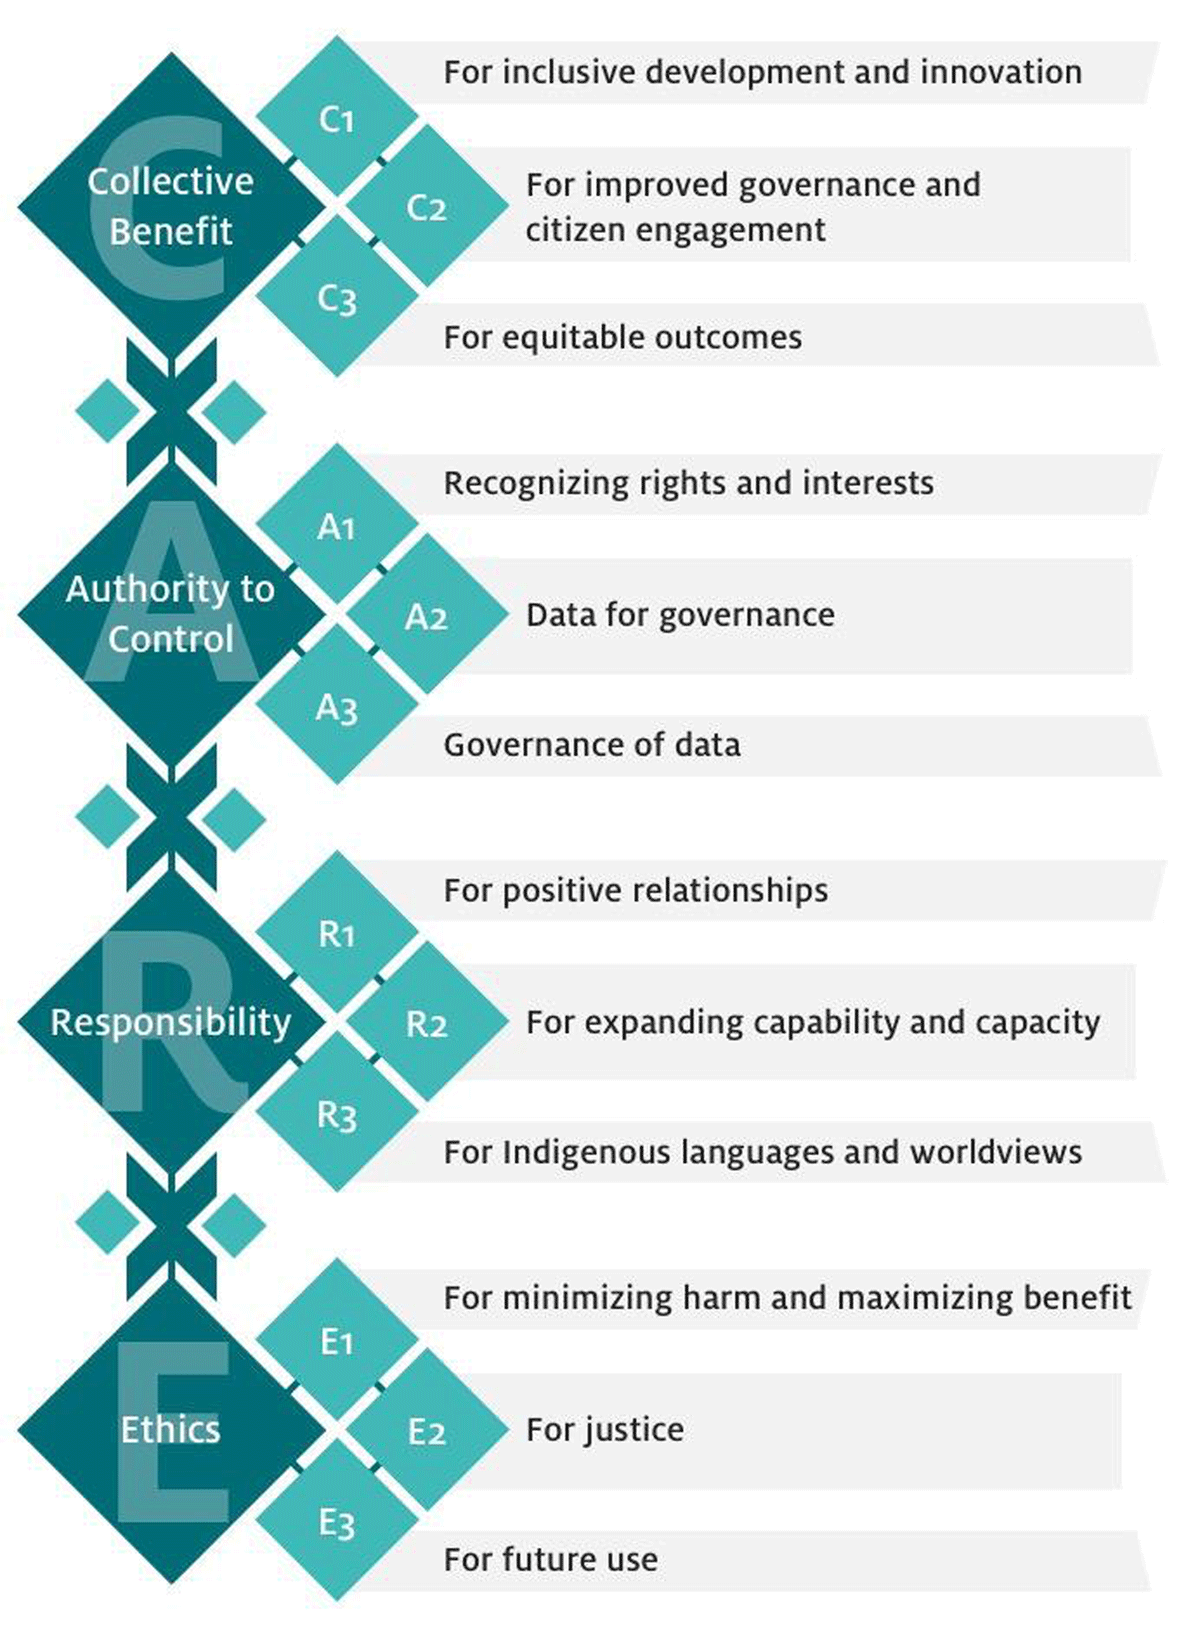
\includegraphics[width=0.43\columnwidth]{figures/CARE-principles.png}
\caption{CARE Principles for Indigenous Data Governance (adapted from \textcite{Carroll2020}, figure 2)}
\vspace{1cm}  % Increase this value to add more space after the figure
\end{wrapfigure}

Local Contexts Notices and Labels have been developed as a system to add cultural context to data and collections. This system allows for the clear communication of Indigenous rights and interests associated with specific data sets or cultural artifacts. Notices are informational text that provide context about the Indigenous provenance and cultural significance of data or collections. They can be applied by institutions or researchers to indicate their recognition of Indigenous rights and interests. Labels, on the other hand, are visual markers created and applied by Indigenous communities themselves. These Labels express community-specific protocols for accessing and using cultural heritage materials. Both Notices and Labels work together to enhance understanding of proper data use, promote ethical research practices, and respect Indigenous cultural protocols throughout the research lifecycle.

However, there are still limitations in specifying how to capture and carry forward this contextual information throughout the entire research lifecycle, from project inception to long-term data preservation and reuse. Current research data management practices often struggle to maintain the connection between Indigenous consent, cultural context, and the data itself as it moves through various stages of research and potentially gets reused in different contexts. This challenge highlights the need for a more robust and persistent method of recording and tracking CARE-related metadata throughout the research process.
}

%----------------------------------------------------------------------------------------
% RAiD
%----------------------------------------------------------------------------------------
\color{ARDCBlue}
\section*{\LARGE The Research Activity Identifier (RAiD)}
\color{DarkGrey}
\large{
The Research Activity Identifier (RAiD) is proposed as a solution to address the challenges of persistently recording CARE Principles and Local Contexts information. RAiD is a persistent identifier and system for research projects and activities, governed by ISO Standard 23527:2022. The Australian Research Data Commons (ARDC) serves as the global Registration Authority and lead developer of the RAiD system.

RAiD functions by linking organizations, people, inputs, and outputs to a project, providing a comprehensive and dynamic record of key project information. This information is often not found in any other single source, making RAiD a valuable tool for research project management and data governance.

The RAiD system offers several key features that make it particularly suitable for implementing the CARE Principles:

\begin{enumerate}
\item Persistent Identification: RAiD provides a stable, long-term identifier for research projects, ensuring that project metadata remains accessible and linked even as research outputs evolve over time.
\item Comprehensive Metadata: RAiD stores, updates, shares, and links project metadata information for the global research community, allowing for the inclusion of CARE-related information and Local Contexts Notices or Labels.
\item Dynamic Updates: The system can handle changes in Indigenous consent or cultural context throughout the project lifecycle, maintaining an up-to-date record of permissions and cultural considerations.
\item Interoperability: RAiD is designed to work alongside other persistent identifiers and research information systems, facilitating the integration of CARE Principles into existing research infrastructure.
\end{enumerate}

Additionally, RAiD offers broader benefits to the research ecosystem. It provides comprehensive project tracking by recording organizations contributing to funding and collection, enabling funders to track impact and return on investment more effectively. The system enhances administrative efficiency by providing a single source of truth for project metadata, reducing administrative burden and minimizing errors that can arise from disparate metadata sources. RAiD also supports FAIR data principles by providing clear provenance for research outputs through project-level metadata, including a comprehensive history of changes. Finally, the system is designed for flexible integration, allowing it to be embedded in existing infrastructure, services, and products used to conduct and manage research, facilitating seamless adoption across different disciplines and contexts.

}

% ---------------------------
% RAiD Diagram
% ---------------------------
% Add vertical space before the diagram
\vspace{2cm}
% Center the diagram using TikZ
\begin{center}
\begin{tikzpicture}[
    node distance = 0.7cm and 4cm,
    box/.style = {rectangle, minimum width=3.2cm, minimum height=0.9cm, text centered, font=\sffamily\small, rounded corners=3pt},
    main/.style = {box, fill=DarkGrey, text=white, font=\sffamily\bfseries\Large},
    category/.style = {box, text=white, font=\sffamily\bfseries\large},
    core/.style = {category, fill=ARDCBlue},
    extended/.style = {category, fill=ARDCPink},
    local/.style = {category, fill=ARDCPurple},
    item/.style = {box, fill=ARDCYellow, text=DarkGrey},
    group/.style = {draw=DarkGrey, dashed, inner sep=12pt, rounded corners=5pt},
    tk/.style = {draw=DarkGrey, line width=1pt, text=DarkGrey}
]
% Use a coordinate system to center the diagram
\path coordinate (origin);
% Main node
\node[main] (raid) at (origin) {RAiD Metadata};
% Three main categories
\node[core, below=1.5cm of raid] (core) {Core};
\node[extended, below left=3cm and 5cm of raid] (extended) {Extended};
\node[local, below right=3cm and 5cm of raid] (local) {Local};
% Core Metadata items
\node[item, below=of core] (c1) {Identifier};
\node[item, below=of c1] (c2) {Title};
\node[item, below=of c2] (c3) {Description};
\node[item, below=of c3] (c4) {Dates};
\node[item, below=of c4] (c5) {Contributors};
\node[item, below=of c5] (c6) {Organisations};
\node[item, below=of c6] (c7) {Related RAiDs};
% Extended Metadata items
\node[item, below=of extended] (e1) {Subjects};
\node[item, below=of e1] (e2) {Alternate Identifiers};
\node[item, below=of e2] (e3) {Access};
\node[item, below=of e3] (e4) {Spatial Coverage};
\node[item, below=of e4, tk] (e5) {TK Labels};
\node[item, below=of e5, tk] (e6) {TK Notices};
% Local Metadata item with forced hyphenation
\node[item, text width=4cm, below=of local] (l1) {\hspace{0pt}Cus\-tom\-is\-able by Reg\-is\-tra\-tion Agency};

% Group boxes using fit and backgrounds
\begin{scope}[on background layer]
    \node[fit=(core) (c1) (c2) (c3) (c4) (c5) (c6) (c7), group] {};
    \node[fit=(extended) (e1) (e2) (e3) (e4) (e5) (e6), group] {};
    \node[fit=(local) (l1), group] {};
\end{scope}
\end{tikzpicture}

% Caption
\parbox{0.8\columnwidth}{
    \captionof{figure}{High-level RAiD metadata elements with Local Contexts TK Labels and Notices highlighted \parencite{RAiDMetadata}.}
}
\end{center}
% ---------------------------
% End RAiD Diagram
% ---------------------------




%----------------------------------------------------------------------------------------
% RAID IMPLEMENTATION
%----------------------------------------------------------------------------------------
\color{ARDCPurple}
\section*{\LARGE RAiD Implementation for CARE Principles}
\color{DarkGrey}
\large{
The implementation of Research Activity Identifiers (RAiDs) offers a promising solution for improving the recording and tracking of CARE Principles and Local Contexts information in research involving Indigenous data. By providing a persistent, comprehensive, and dynamic system for managing project metadata, RAiD addresses many of the current challenges in ensuring ethical and responsible research practices.

The implementation of RAiD offers several significant benefits:

\begin{enumerate}
\item Declaration of Traditional Knowledge or Biocultural Notices and Labels: RAiD can be used to declare and link to relevant Local Contexts Notices or Labels, ensuring that cultural context and Indigenous rights are clearly associated with the research project and its outputs.
\item Documentation Linkage: The system can link to documents describing sampling and field data acquisition circumstances, providing crucial context for the ethical collection and use of Indigenous data.
\item Consistency in Downstream Use: By maintaining persistent links between the project identifier and its various outputs (e.g., subsamples, datasets, and publications), RAiD ensures that CARE-related information remains associated with research data throughout its lifecycle.
\item Consent Management: The dynamic nature of RAiD allows for the recording and tracking of changes in Indigenous consent over time, providing a clear history of permissions and any modifications to data usage agreements.
\item CARE-related Metadata: RAiD allows for the inclusion of CARE-related information and Local Contexts Notices or Labels in its comprehensive metadata.
\item Indigenous Consent Tracking: The system can handle changes in Indigenous consent or cultural context throughout the project lifecycle, maintaining an up-to-date record of permissions and cultural considerations.
\end{enumerate}

The adoption of RAiD can significantly enhance the ability of researchers and institutions to respect Indigenous Data Sovereignty, maintain proper consent records, and ensure that cultural context remains associated with data throughout its lifecycle. This approach not only benefits Indigenous communities by protecting their rights and interests but also supports the broader research community by improving data provenance, facilitating collaboration, and enhancing the overall quality and ethical standards of research.

As the research landscape continues to evolve, tools like RAiD will play a crucial role in fostering trust, transparency, and respect between researchers and Indigenous communities. By persistently recording and honoring the CARE Principles, we can work towards a more equitable and ethical approach to research that truly benefits all stakeholders.
}

\vfill

%----------------------------------------------------------------------------------------
% REFERENCES
%----------------------------------------------------------------------------------------
\color{ARDCBlue}
\section*{\LARGE References}
\color{DarkGrey}
\large{
\printbibliography[heading=none]
}


\vfill

%----------------------------------------------------------------------------------------
% LICENSE
%----------------------------------------------------------------------------------------
\begin{center}
\begin{tabular}{cc}
\raisebox{-0.2\height}{
\includegraphics[height=1cm]{cc-by.png}} &
\raisebox{0.2ex}{\small This work is licensed under a Creative Commons Attribution 4.0 International License.}
\end{tabular}
\end{center}




\end{multicols}

\end{document}